\chapter{Simulations Monte-Carlo}
\label{ch-mc}

Une prédiction décrit le réseau en chaque point, pour une charge fixée à l'avance. Une simulation Monte-Carlo place de vrais utilisateurs : Atoll les tire au hasard selon la carte de trafic, calcule pour chacun son serveur, son SINR, son bearer et son débit, ainsi que la charge de chaque cellule, puis répète le tirage pour obtenir des statistiques. Le sujet demande des simulations pour 10, 100 et \num{1000} utilisateurs et leur fonction de distribution cumulative inverse (DCFI) sur un même graphique.

\section{Paramétrage}

\begin{itemize}
  \item \textbf{Nombre d'utilisateurs :} la carte de trafic contient \num{25359} utilisateurs potentiels (un par habitant). Le facteur d'échelle global de chaque groupe vaut $N / \num{25359}$, soit \SI{0,0394}{\percent}, \SI{0,394}{\percent} et \SI{3,94}{\percent} pour 10, 100 et \num{1000} utilisateurs. Les trois groupes partagent ainsi la même carte : leurs courbes sont comparables.
  \item \textbf{Répétitions :} 20 simulations par groupe ; charge maximale de \SI{80}{\percent} en DL et en UL ; paramètres de convergence par défaut.
  \item \textbf{Graine du générateur :} fixée à 1, ce qui rend les tirages reproductibles. Cette propriété sert au \cref{ch-opt} : les mêmes utilisateurs sont tirés sur le réseau initial et sur le réseau final.
\end{itemize}

Un utilisateur actif du service High Speed Internet demande environ \SI{1}{\Mbps} ; la demande de l'heure chargée calculée à l'Étape 1 (\SI{225}{\Mbps} en ville) correspond donc à quelques centaines d'utilisateurs simultanés. 10 utilisateurs représentent donc un réseau presque vide, 100 une charge normale et \num{1000} un test de stress au-delà de l'heure chargée.

\section{Résultats par groupe}

\begin{table}[H]
\centering
\caption{Résultats Monte-Carlo (moyenne de 20 tirages).}
\label{tab-mc}
\begin{tabular}{@{}lccc@{}}
\toprule
\thead{Indicateur} & \thead{MC-10} & \thead{MC-100} & \thead{MC-1000} \\
\midrule
Utilisateurs tirés (écart-type) & 9,95 (3,0) & 100 (11,3) & \num{1001,6} (35,6) \\
Rejetés & \SI{8,5}{\percent} & \SI{9,5}{\percent} & \SI{10,8}{\percent} \\
\quad dont pas de couverture / pas de service & 0,30 / 0,55 & 2,35 / 7,2 & 26,6 / 81,7 \\
\quad dont saturation & 0 & 0 & 0 \\
Demande DL & \SI{6,06}{\Mbps} & \SI{64,4}{\Mbps} & \SI{650,9}{\Mbps} \\
Débit DL servi (applicatif, cumulé) & \SI{4,23}{\Mbps} & \SI{40,2}{\Mbps} & \SI{257,3}{\Mbps} \\
Débit UL servi (applicatif, cumulé) & \SI{0,68}{\Mbps} & \SI{6,85}{\Mbps} & \SI{68,3}{\Mbps} \\
\bottomrule
\end{tabular}
\end{table}

Le nombre d'utilisateurs tirés varie autour de la demande : pour MC-10, la moyenne vaut 9,95 et l'écart-type 3,04, proche de $\sqrt{10} \approx 3{,}16$, ce qui correspond à un tirage de Poisson. Pour la demande DL de MC-10, le mélange de services donne $0{,}60 × 1024 + 0{,}25 × 128 + 0{,}15 × 12{,}2 \approx \SI{648}{\kbps}$ par utilisateur, soit environ \SI{6,4}{\Mbps} pour 9,95 utilisateurs, du même ordre que les \SI{6,06}{\Mbps} d'Atoll.

\section{Pourquoi des utilisateurs sont rejetés}
\label{sec-tests}

Atoll fait passer à chaque utilisateur tiré trois tests successifs ; la fenêtre de statistiques d'Atoll (\cref{fig-mc}b) donne le nombre d'échecs à chacun :
\begin{enumerate}
  \item Le signal arrive-t-il ? Au moins une cellule doit être reçue au-dessus du seuil de réception. Sinon : \enquote{pas de couverture}.
  \item Le signal est-il assez propre ? Le C/(I+N) doit atteindre le seuil du bearer le plus robuste, \SI{-1}{\deci\bel}. Sinon : \enquote{pas de service}. Ce seuil se lit dans les données exportées : tous les utilisateurs connectés ont un C/(I+N) d'au moins \SI{-0,9}{\deci\bel}, tous les \enquote{pas de service} au plus \SI{-1,1}{\deci\bel}.
  \item La cellule a-t-elle de la place ? Il doit rester des ressources radio (charge maximale de \SI{80}{\percent}). Sinon : saturation.
\end{enumerate}

\begin{figure}[H]
\centering
\begin{subfigure}[b]{0.56\textwidth}\centering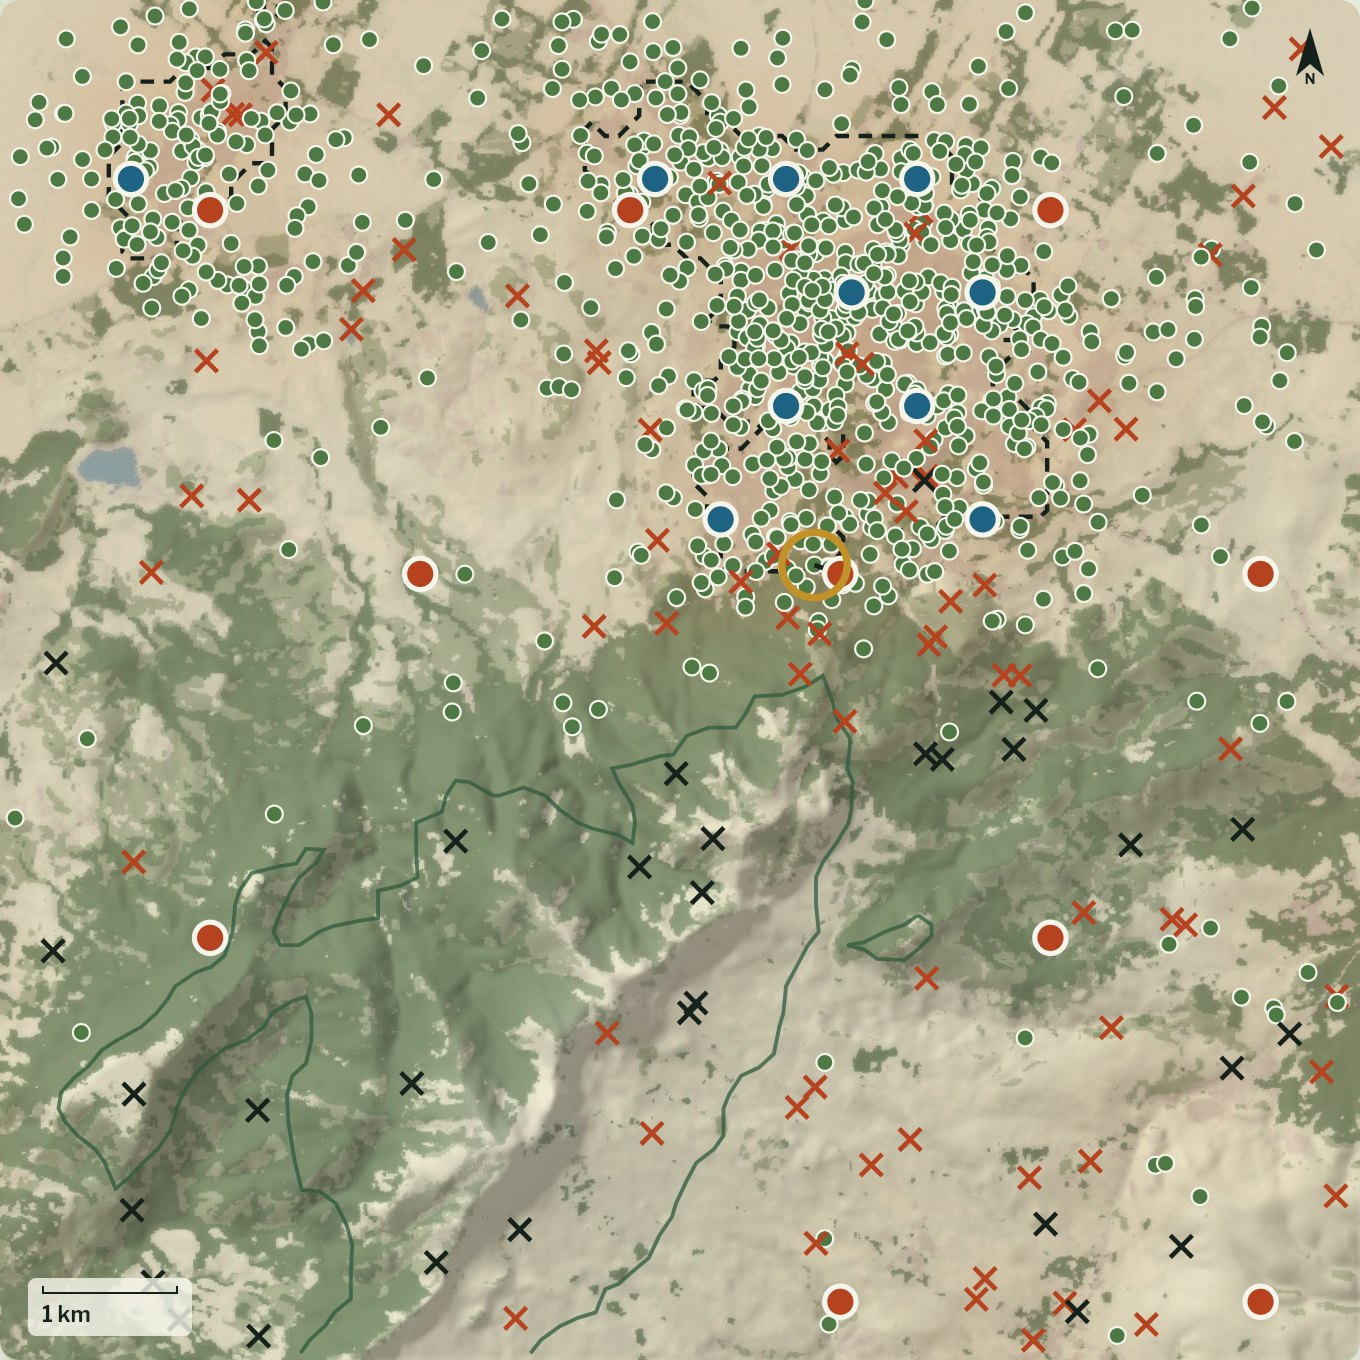
\includegraphics[width=\textwidth]{mc-tests.jpg}\caption{Un tirage de MC-1000.}\end{subfigure}\hfill
\begin{subfigure}[b]{0.42\textwidth}\centering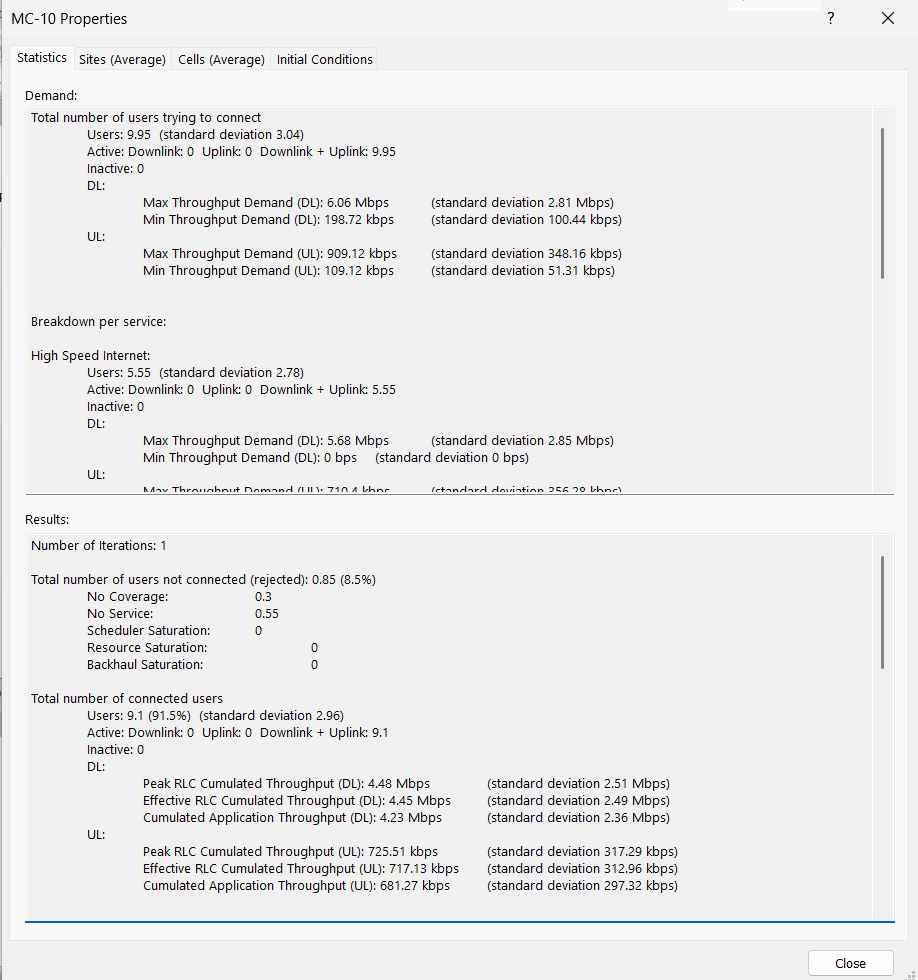
\includegraphics[width=\textwidth]{S04-05_MC10_statistiques.png}\caption{Statistiques d'Atoll (MC-10).}\end{subfigure}
\caption{Utilisateurs simulés et causes de rejet.}
\label{fig-mc}
\end{figure}

Sur la \cref{fig-mc}a, les utilisateurs connectés sont en vert, les \enquote{pas de couverture} en croix noires et les \enquote{pas de service} en croix rouges ; les sites urbains et ruraux sont en bleu et en terre cuite. Dans ce tirage de \num{1041} utilisateurs, 31 échouent au test 1, 77 au test 2 et \textbf{aucun au test 3} ; 933 sont connectés. Sur les 20 tirages, le taux de saturation est nul pour les trois groupes. Tous les rejets viennent donc du signal (couverture et interférence), aucun de la capacité. Les 108 rejetés se répartissent en 76 dans la campagne loin des sites, 14 sur le massif et 18 en ville, dont 17 à l'intérieur des bâtiments, où \SI{15}{\deci\bel} de pénétration s'ajoutent à l'interférence entre sites urbains.

\section{La DCFI}
\label{sec-dcfi}

La DCFI est la fonction de distribution cumulative inverse (ou complémentaire) du débit : pour chaque débit $x$, elle donne la proportion des utilisateurs qui obtiennent au moins $x$,
\begin{equation}
  \text{DCFI}(x) = P(\text{débit} \geq x) = 1 - F(x),
\end{equation}
où $F$ est la fonction de répartition. Pour un débit choisi sur l'axe horizontal, la courbe donne la part des utilisateurs servis au moins à ce débit. Nous l'avons tracée à partir du débit applicatif de \emph{chaque} utilisateur, exporté d'Atoll (onglet \enquote{Mobiles} des simulations), en comptant les utilisateurs rejetés à \SI{0}{\kbps}. Les courbes portent sur les utilisateurs du service High Speed Internet, celui qui porte l'objectif de bord de cellule.

Échantillons utilisés : MC-10, les 20 tirages (199 utilisateurs, dont 111 HSI) ; MC-100, 5 tirages (528, dont 326 HSI) ; MC-1000, 2 tirages (\num{2104}, dont \num{1224} HSI). Leur taux de rejet (\SI{8,5}{\percent}, \SI{9,3}{\percent}, \SI{10,5}{\percent}) est proche de la moyenne des 20 tirages : les échantillons sont représentatifs.

\begin{figure}[H]
\centering
\begin{subfigure}[b]{0.49\textwidth}\centering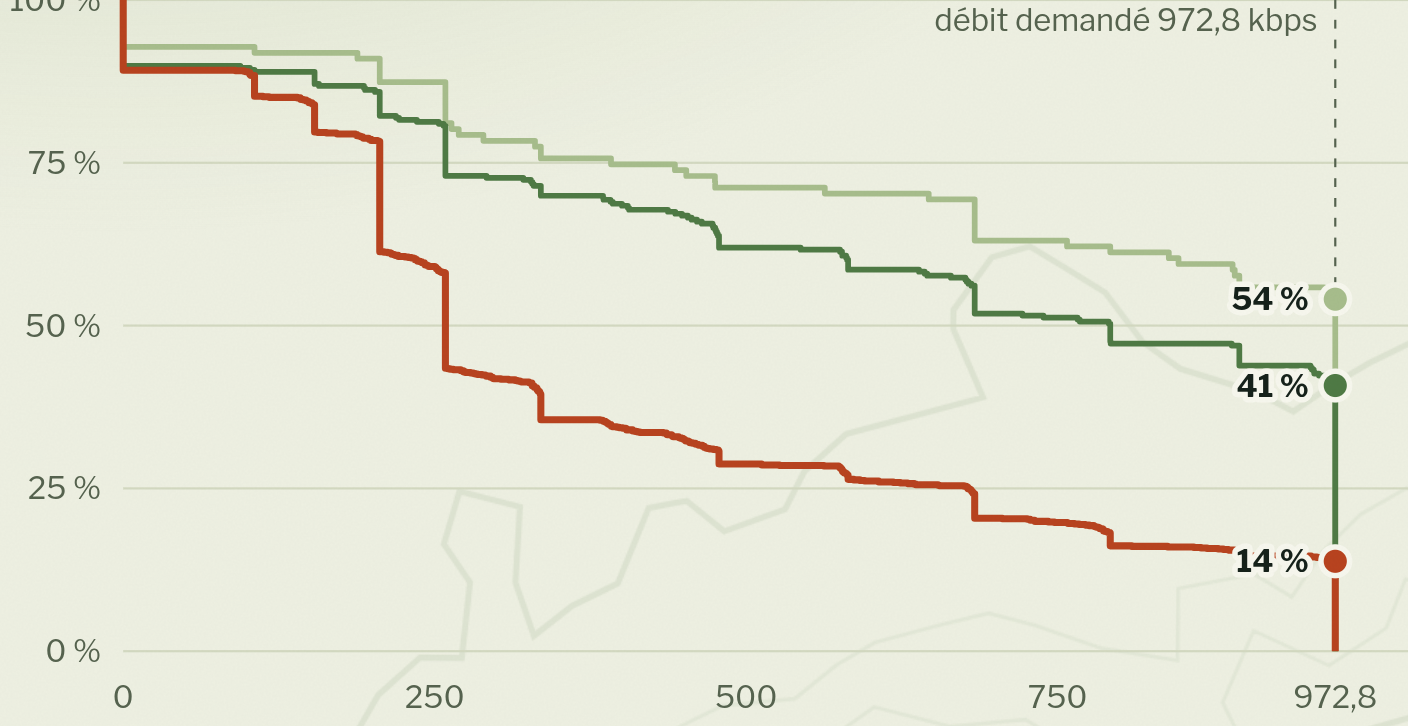
\includegraphics[width=\textwidth]{dcfi-dl.png}\caption{DL.}\end{subfigure}\hfill
\begin{subfigure}[b]{0.49\textwidth}\centering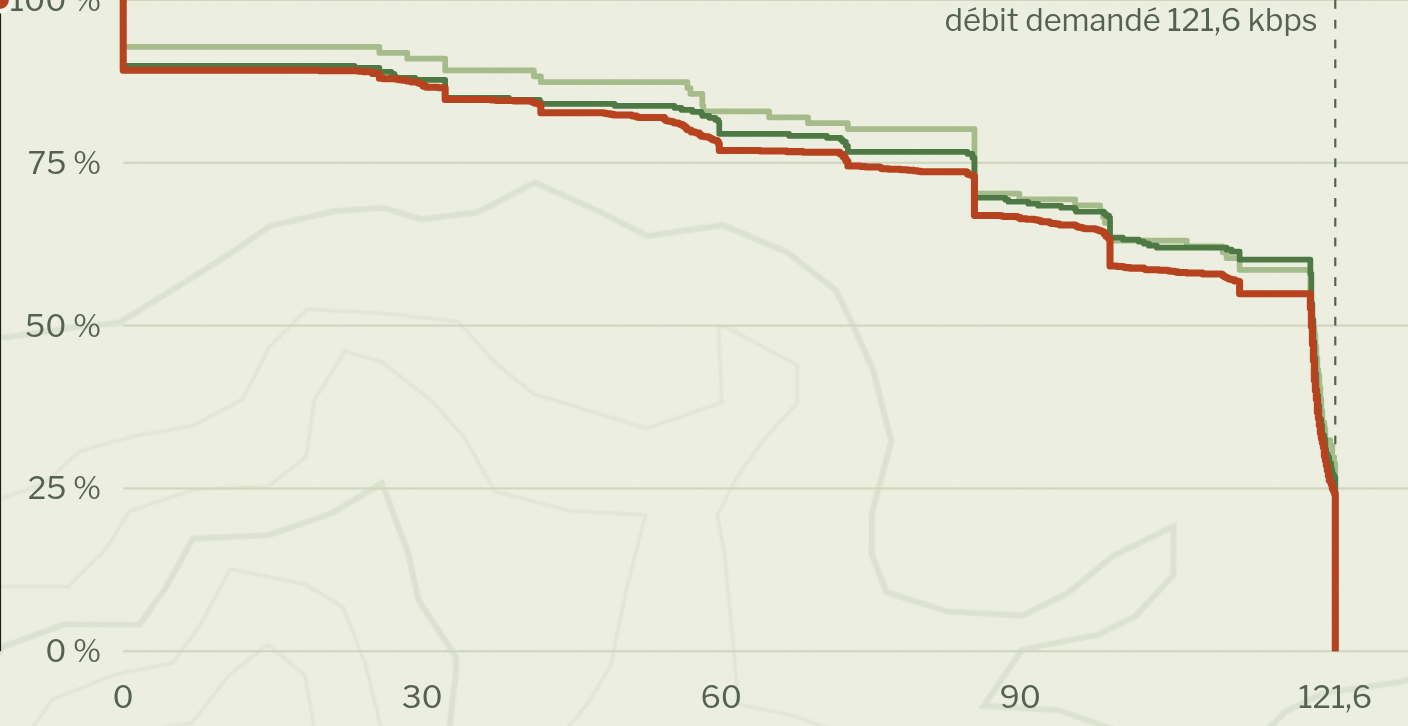
\includegraphics[width=\textwidth]{dcfi-ul.png}\caption{UL.}\end{subfigure}
\caption{DCFI du débit applicatif des utilisateurs HSI.}
\label{fig-dcfi}
\end{figure}

Sur la \cref{fig-dcfi}, les courbes de 10, 100 et \num{1000} utilisateurs sont en vert clair, en vert et en terre cuite. Le débit demandé vaut \SI{972,8}{\kbps} en DL et \SI{121,6}{\kbps} en UL : ce sont les débits applicatifs $1024 × 0{,}95$ et $128 × 0{,}95$.

\begin{table}[H]
\centering
\caption{Lecture des DCFI (utilisateurs HSI).}
\label{tab-dcfi}
\begin{tabular}{@{}lccc@{}}
\toprule
\thead{Indicateur} & \thead{MC-10} & \thead{MC-100} & \thead{MC-1000} \\
\midrule
Part au débit demandé en DL & \SI{54}{\percent} & \SI{41}{\percent} & \textcolor{terre}{\textbf{\SI{14}{\percent}}} \\
Débit DL médian & \SI{973}{\kbps} & \SI{792}{\kbps} & \textcolor{terre}{\textbf{\SI{259}{\kbps}}} \\
Part au débit demandé en UL & \SI{32}{\percent} & \SI{29}{\percent} & \SI{26}{\percent} \\
Tous services : part servie au débit demandé en DL & \SI{59}{\percent} & \SI{47}{\percent} & \SI{25}{\percent} \\
\bottomrule
\end{tabular}
\end{table}

\section{Synthèse et impact sur le dimensionnement}
\label{sec-p4}

Les courbes se lisent en trois points.
\begin{enumerate}
  \item À $x = 0$, les trois courbes partent d'environ \SI{90}{\percent} : environ \SI{10}{\percent} des utilisateurs sont rejetés quel que soit leur nombre, tous pour une raison de signal. Ce problème de couverture est la cible de l'optimisation.
  \item Le débit DL médian passe de 973 à \SI{259}{\kbps} de 10 à \num{1000} utilisateurs. Le service est \enquote{best effort} : faute de place, Atoll donne moins de débit à l'utilisateur au lieu de le rejeter. Le DL est donc limité par la capacité et l'interférence.
  \item Les trois courbes UL sont presque superposées. L'UL est limité par la puissance du terminal, comme l'annonçait le bilan de liaison (liaison montante limitante de \SI{2}{\deci\bel}).
\end{enumerate}

Ces résultats confirment l'Étape 1 sur deux points : la liaison montante limite la couverture, et la capacité n'est pas le facteur dimensionnant aujourd'hui (aucune saturation, même à \num{1000} utilisateurs). Ils précisent aussi la limite de capacité : à \num{1000} utilisateurs simultanés, la médiane tombe à \SI{259}{\kbps}. L'objectif de \SI{1}{\Mbps} tient pour quelques centaines d'utilisateurs simultanés, ce qui couvre la demande actuelle de l'heure chargée ; au-delà, il faudra ajouter de la capacité (une seconde porteuse ou de petites cellules) et non de la couverture.

Un résultat reste inexpliqué : même dans MC-10, \SI{46}{\percent} des utilisateurs HSI reçoivent moins de \SI{1}{\Mbps} alors qu'ils sont seuls dans leur cellule avec un bon C/I (médiane d'environ \SI{20}{\deci\bel}). Ce n'est expliqué ni par la mobilité ni par le nombre d'utilisateurs par cellule ; il s'agit probablement d'une règle interne de l'ordonnanceur d'Atoll, que nous n'avons pas pu vérifier. Nous la signalons parmi les limites (\cref{sec-limites}).
